\documentclass{article}
\usepackage[final,sglblindworkshop]{neurips_2026}
\workshoptitle{Dynamic Alignment in Human-AI Coupled System}
\makeatletter
\renewcommand{\@noticestring}{40th Conference on Neural Information Processing Systems (NeurIPS 2026). Workshop: Dynamic Alignment in Human-AI Coupled System}
\makeatother
\usepackage[utf8]{inputenc}
\usepackage[T1]{fontenc}
\usepackage{amsmath,amssymb,amsthm,booktabs,graphicx,hyperref,microtype,xcolor}
\hypersetup{colorlinks=true,linkcolor=blue,citecolor=blue,urlcolor=blue,pdfauthor={Lakshya Narula},pdftitle={Who Keeps Giving Feedback? Participation Feedback Creates Alignment Lock-In}}
\newtheorem{proposition}{Proposition}
\newcommand{\sigmoid}{\sigma}
\title{Who Keeps Giving Feedback?\\Participation Feedback Creates Alignment Lock-In}
\author{Lakshya Narula\\University of Minnesota-Twin Cities\\\texttt{narul014@umn.edu}}
\begin{document}
\maketitle
\begin{abstract}
A deployed alignment policy can change who supplies its next round of feedback. If better service elicits greater participation from one group, feedback-based updates can amplify an initial imbalance even when preferences do not change. Building on prior models of performance-dependent user retention, we study representative recruitment as an intervention in this loop. A two-group model yields an exact threshold: the representative policy is globally attracting when the feedback gain is at most 1, but two unrepresentative attractors appear above that threshold. At the equality boundary, convergence remains stable but becomes polynomially slow. We derive how unequal population shares, biased audit feedback, delayed responses, and finite feedback change this conclusion. Simulations separate across-deployment averages from within-deployment lock-in and show when a local noise approximation is informative. The resulting measurement protocol distinguishes a policy's effect on response propensity from its effect on preferences. Representative feedback is not just an evaluation sample: its effective weight and sampling quality can determine the stability of the alignment process itself.
\end{abstract}

\section{Alignment can choose its future feedback providers}
Feedback learning links deployment to training. Human comparisons guide reward learning and policy updates~\citep{christiano2017,ouyang2022,bai2022,rafailov2023}; the resulting system then determines which experiences users evaluate. Much attention has gone to aggregating heterogeneous preferences~\citep{conitzer2024,ge2024}, representing multiple reward functions~\citep{chakraborty2024}, and protecting groups within preference data~\citep{ramesh2024,kim2026}. A distinct design question concerns the boundary of the dataset: \emph{does today's policy change who supplies tomorrow's feedback?}

Imagine two equally numerous groups that prefer different assistant behaviors. A small initial policy advantage makes giving feedback more worthwhile for the better-served group. The next training set then overrepresents that group, encouraging a further policy shift. Both groups can be truthful and their preferences can remain fixed throughout. An apparently stable policy may therefore reflect a stable participation imbalance rather than representative support. Tracking total feedback volume does not necessarily reveal the problem: one group's increased participation can offset another's decline.

\citet{hashimoto2018} model prediction losses changing user retention and show how repeated empirical risk minimization can disadvantage minority groups. Performative prediction supplies a general framework for predictors changing their subsequent data distribution~\citep{perdomo2020}. Building on these foundations, we ask what weight on an independently representative feedback stream stabilizes participation-sensitive alignment, and what a finite, imperfect audit can guarantee.

The mechanism fits the model-dependent distribution maps surveyed by \citet{survey2025}. Prior work separates training steps from deployments~\citep{mendler2020} and allows population responses to depend on earlier distributions~\citep{brown2022}. We expose a recruitment weight within the coupled update. In predictive policing, \citet{ensign2018} distinguish deployment-dependent discoveries from externally reported incidents. Our representative stream plays a related corrective role; its guarantees concern the logistic response, exact stability threshold, and audit error.

The distinction is relevant to current feedback systems. \citet{de2026} document substantial rater attrition and selected participation in artificial-intelligence-assisted Community Notes; among tweets with at least two collaborative-note versions, first-to-second-version rater retention is 40.9\%. This observational finding motivates measuring participation separately from preferences, but does not estimate our causal loop. Recruitment of diverse and partly census-representative feedback providers for the PRISM alignment dataset similarly emphasizes that the observed electorate is a design choice~\citep{kirk2024}. Neither study supplies our response parameter.

Our contributions are the global threshold including its equality case, extensions to unequal populations and imperfect audits, finite-feedback analysis, and a causal measurement protocol.

\section{A model of service, participation, and updating}\label{sec:model}
Two groups have fixed preferred policies, 1 and 0. The scalar $x_t\in[0,1]$ is the share of deployed service allocated to group 1 at round $t$; the remaining share serves group 2. One implementation is randomization between two fixed response policies. We call $x=1/2$ representative for an equally sized population. This is a declared proportional-service target, not a theorem that equal mixing maximizes welfare for every application. The model tracks deployment-level allocation rather than individual neural-network weights.

Let $r_1(x)$ and $r_2(x)$ be response probabilities conditional on an invitation. In the symmetric model assume
\begin{equation}
\frac{r_1(x)}{r_2(x)}=\exp\{\beta(2x-1)\},\qquad \beta\ge0.
\label{eq:ratio}
\end{equation}
The parameter $\beta$ measures how own-group service changes relative willingness or ability to provide feedback. A concrete admissible realization is $r_1(x)=\sigma(\beta(2x-1))$ and $r_2(x)=1-r_1(x)$, where $\sigma(z)=(1+e^{-z})^{-1}$. These probabilities could reflect differences in expected influence, task relevance, or effort; no strategic misreporting is assumed. Equal invitation rates and equal population shares imply that group 1's share among respondents is
\begin{equation}
p(x)=\frac{r_1(x)}{r_1(x)+r_2(x)}=\sigma(\beta(2x-1)).
\label{eq:participation}
\end{equation}
In the concrete realization the aggregate response probability is always $1/2$, even as the respondent mix changes. A count-only participation dashboard would miss this selection entirely.

The provider combines the endogenous stream with an independently representative stream. Let $\alpha\in[0,1]$ be the latter's \emph{effective weight} in the update target. With exact representative composition and adjustment rate $\lambda\in(0,1]$,
\begin{equation}
x_{t+1}=F(x_t)=(1-\lambda)x_t+\lambda\left[(1-\alpha)p(x_t)+\alpha/2\right].
\label{eq:update}
\end{equation}
Here $\lambda$ describes partial policy adjustment, not the participation parameter. An audit stream may be a recruited panel or an independently sampled population survey. Its weight can be set by reweighting and need not equal its raw sample-count fraction. Recruiting nominally representative invitees is insufficient if selective nonresponse remains uncorrected; the assumed quantity is representative \emph{feedback entering the update}.

Equation~\eqref{eq:update} deliberately uses a proportional feedback-to-policy rule. Population-proportional alignment and social-choice analyses motivate studying representation guarantees~\citep{kim2026,ge2024,fish2025}, but ordinary reinforcement learning from human feedback (RLHF) or direct preference optimization (DPO) does not in general implement this scalar rule. Applying the threshold to a trained model therefore requires measuring the local response of deployed policy to feedback composition. Section~\ref{sec:measurement} explains that calibration. Our theorem describes a transparent coupled-system mechanism, not a guarantee for an unspecified optimizer.

\paragraph{Selection versus preference or strategy.}
The groups' evaluations of policies do not move in this model; their probabilities of being observed do. Algorithmic confounding and recommender feedback can instead change observed behavior or user interests~\citep{chaney2018,jiang2019}. Strategic data annotation~\citep{xie2024}, coordinated data modification~\citep{hardt2023}, and strategyproof preference learning~\citep{kleine2025,sun2025} concern additional channels. Recursive curation studies another long-horizon coupling between learners and generated content~\citep{falahati2026}. These mechanisms can coexist with participation selection. They are not competing explanations that our stylized model rules out.

Recursive training on generated data can also lose distributional information through repeated sampling and approximation~\citep{shumailov2024}. Our instability requires neither generated labels nor finite-sample error: it occurs in the deterministic, truthful-response model. In the terminology of \citet{suresh2021}, the central concern is who enters the sample, distinct from whether the recorded label measures the intended preference.

\section{When representative alignment becomes unstable}\label{sec:threshold}
A fixed point satisfies $F(x^*)=x^*$: the update leaves it unchanged. It is attracting if nearby trajectories approach it, and globally attracting if every initial policy does so. Stability additionally means sufficiently small perturbations remain small. A bifurcation is a change in this fixed-point structure as a parameter varies. We use these terms for the stated deterministic update, not as labels for observed human behavior.
Define the dimensionless feedback gain $\gamma=(1-\alpha)\beta/2$. The derivative at the representative point is
\begin{equation}
d=F'(1/2)=1-\lambda+\lambda\gamma.
\label{eq:gain}
\end{equation}
The quantity $\gamma$ multiplies the participation response by the weight placed on endogenous feedback. The adjustment rate determines how fast this gain acts, but not whether it exceeds one.

\begin{proposition}[Global threshold and critical stability]\label{prop:threshold}
For Eq.~\eqref{eq:update}, if $\gamma\le1$, the representative fixed point is unique and globally asymptotically stable. If $\gamma<1$, $F$ is a contraction: it multiplies distances by at most a factor $d<1$, so $|F(x)-F(z)|\le d|x-z|$. At $\gamma=1$, convergence is asymptotic but not exponentially fast. If $\gamma>1$, the representative point is unstable and exactly two asymmetric attracting fixed points exist; every initial point strictly above or below $1/2$ converges to the fixed point on its respective side.
\end{proposition}
\emph{Proof.} Set $y=2x-1$ and $a=1-\alpha$. The update becomes
\begin{equation}
y_{t+1}=H(y_t)=(1-\lambda)y_t+\lambda a\tanh(\beta y_t/2),
\quad y^*=a\tanh(\beta y^*/2).
\label{eq:fixed}
\end{equation}
Here $\tanh z=(e^z-e^{-z})/(e^z+e^{-z})$ is the hyperbolic tangent; below, $\sinh z=(e^z-e^{-z})/2$ is the hyperbolic sine. For $y>0$, $\tanh(\beta y/2)<\beta y/2$ whenever $\beta>0$. Thus for $\gamma\le1$ every positive iterate decreases toward zero, while odd symmetry gives the analogous result for negative iterates. The cases $a=0$ or $\beta=0$ reduce to a linear contraction. Since $0\le H'(y)\le1-\lambda+\lambda\gamma$, strict inequality gives the global contraction claim. At $\gamma=1$, strict decrease still proves convergence, although the derivative at zero equals one.

If $\gamma>1$, the function $a\tanh(\beta y/2)-y$ has positive derivative at zero, is strictly concave for positive $y$, and is negative at $y=1$. It therefore has exactly one positive zero $y_+$ and, by odd symmetry, exactly one negative zero. At a nonzero root, put $z=\beta|y_+|/2>0$. The target derivative equals $2z/\sinh(2z)<1$, so the update derivative lies in $[0,1)$. The monotonicity of $H$ prevents crossing a fixed point; its sign relative to $y$ moves every positive initial point toward $y_+$ and every negative point toward $-y_+$. $\square$

For $\beta>2$, the smallest deterministic stabilizing audit weight is $\alpha_c=1-2/\beta$. Equality is stable, not unstable. A strictly larger weight creates a contraction margin and is preferable when estimates or sampling are imperfect. If $\beta\le2$, the symmetric system needs no positive floor for asymptotic stability; this does not imply that feedback is representative at every finite time.

\paragraph{Why slowing updates is insufficient.}
Reducing $\lambda$ moves $d$ toward one from either side. When $\gamma>1$, it slows divergence but leaves the representative point unstable. When $\gamma<1$, it slows convergence. Near a stable fixed point, a perturbation behaves approximately as $d^t$; a convenient local half-life is $\log(1/2)/\log d$ for $0<d<1$. A short evaluation window can mistake slow instability for stability, or slow repair for an ineffective intervention.

\paragraph{The equality boundary.}
At $\gamma=1$, Taylor expansion of Eq.~\eqref{eq:fixed} gives
\begin{equation}
y_{t+1}=y_t-\frac{\lambda\beta^2}{12}y_t^3+O(y_t^5),\qquad
|y_t|\sim\sqrt{\frac{6}{\lambda\beta^2t}}.
\label{eq:critical}
\end{equation}
For a nonzero initial point, monotone convergence gives $y_t\to0$; expanding $y_{t+1}^{-2}-y_t^{-2}$ then gives limit $\lambda\beta^2/6$, establishing the asymptotic expression. The threshold is therefore not a discontinuity between convergence and nonconvergence at equality. It separates a unique representative attractor from a pair of unrepresentative ones, with unusually slow recovery at the boundary.

\begin{figure}[t]\centering
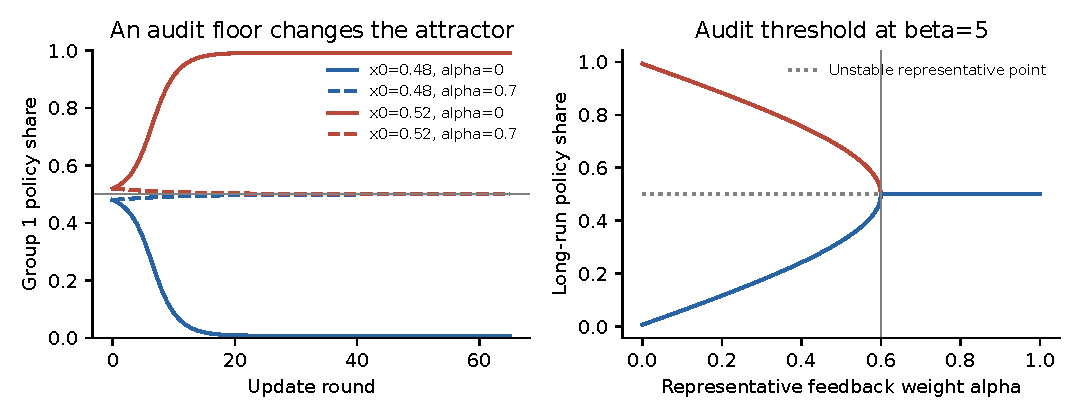
\includegraphics[width=\linewidth]{../results/accepted/participation_phase.pdf}
\caption{Deterministic model, $\beta=5$, $\lambda=.35$. Left: initial shares $.48$ and $.52$ separate without an audit but return to parity at $\alpha=.7$. Right: attractors approached from opposite initial states as the audit weight changes. The critical weight is $.6$; the representative point is unstable below it. Curves are numerical iterations of the stated equations, not deployment observations.}
\label{fig:phase}
\end{figure}

This familiar pitchfork-shaped dynamic translates response sensitivity and effective recruitment weight into a stability requirement. It distinguishes slowing updates from changing feedback gain, for an explicitly chosen proportional target under endogenous observation.

\section{Unequal groups and imperfect representative feedback}\label{sec:extensions}
Equal populations isolate the mechanism but are not necessary for a local analysis. Let group 1's population share be $w\in(0,1)$ and let $r_1,r_2$ be differentiable, positive response rates near the desired policy $x=w$. With common invitation probabilities,
\begin{equation}
p_w(x)=\frac{wr_1(x)}{wr_1(x)+(1-w)r_2(x)},\qquad
F_w(x)=(1-\lambda)x+\lambda[(1-\alpha)p_w(x)+\alpha w].
\label{eq:unequal}
\end{equation}
Assume $r_1(w)=r_2(w)$, so that the representative target is a fixed point. This calibration is substantive: unequal participation at the desired policy would create a level bias before considering dynamic amplification.

\begin{proposition}[Local gain for unequal populations]\label{prop:unequal}
Write $\eta=(\log r_1)'(w)-(\log r_2)'(w)$. Then
\begin{equation}
F_w'(w)=1-\lambda+\lambda(1-\alpha)w(1-w)\eta.
\label{eq:unequalgain}
\end{equation}
If $\eta\ge0$, the representative point is locally exponentially stable when $(1-\alpha)w(1-w)\eta<1$, and unstable when this product exceeds one. Equality requires higher-order analysis.
\end{proposition}
\emph{Proof.} The log odds of $p_w(x)$ equal $\log(w/(1-w))+\log(r_1(x)/r_2(x))$. Differentiating the logistic function gives $p_w'(w)=w(1-w)\eta$, and substituting into the update gives Eq.~\eqref{eq:unequalgain}. Under $\eta\ge0$ the derivative is nonnegative; the ordinary one-dimensional stability criterion gives the strict cases. $\square$

For the centered logistic specialization $p_w(x)=\sigma(\log(w/(1-w))+2\beta(x-w))$, the local gain is $2(1-\alpha)\beta w(1-w)$. At $w=1/2$ this recovers Proposition~\ref{prop:threshold}. Because $w(1-w)$ falls toward the population extremes, this particular local sensitivity can be smaller for an unequal population. That is not a fairness advantage: a small group's absolute representation may still be poor, and local stability does not exclude remote attractors. A global sufficient condition for this logistic specialization is still $(1-\alpha)\beta/2<1$, because $p_w'(x)\le\beta/2$ everywhere.

\paragraph{Local repair can leave a distant attractor.}
Take $w=.2$, $\beta=5$, and $\alpha=.5$. The local feedback gain at the representative policy is $.8$, below one. Nevertheless, the fixed-point equation has roots approximately $.2000$, $.2878$, and $.5423$. The first and third are attracting and the middle is repelling. Thus a locally stable proportional target can coexist with a distant state that overrepresents group 1. Increasing $\alpha$ to $.7$ satisfies the global contraction condition and leaves only $x=.2$. The reproducibility script brackets these roots on a grid and refines them by bisection; substituting them into Eq.~\eqref{eq:unequal} checks their residuals. The example explains why an operating-point experiment cannot establish global safety against large distribution shifts.

\paragraph{A biased audit can be amplified.}
Return to equal populations, but let the effective audit share be $q=1/2+\delta\in[0,1]$. The target is now $(1-\alpha)p(x)+\alpha q$. Under $\gamma<1$ the map remains globally contractive and has a unique fixed point $x_\delta$. Subtracting the unbiased fixed-point equation and using the Lipschitz bound for $p$ gives
\begin{equation}
|x_\delta-1/2|\le \frac{\alpha|\delta|}{1-\gamma},\qquad
\left.\frac{\partial x_\delta}{\partial\delta}\right|_{\delta=0}
=\frac{\alpha}{1-\gamma}.
\label{eq:bias}
\end{equation}
The second equality follows by implicit differentiation, and shows that the first-order sensitivity is sharp. At $\alpha=1$, the fixed point equals $q$ exactly. Close to the critical boundary, a small audit error can be amplified substantially. Stability of the update therefore does not certify accuracy of its target population.

This distinguishes two practical failures. An insufficient audit weight can leave multiple attractors even with an unbiased panel. An adequately weighted but biased panel can produce a unique, stable, unrepresentative attractor. The corresponding remedies differ: the first requires reducing endogenous feedback gain; the second requires improving the population frame, invitation design, or nonresponse correction. Simply increasing the number of observations from the same biased frame does not remove its level error.

\paragraph{One-round delay.}
If endogenous feedback in round $t$ responds to $x_{t-1}$, the local perturbation $e_t=x_t-1/2$ obeys $e_{t+1}=(1-\lambda)e_t+\lambda\gamma e_{t-1}$. Its characteristic polynomial is $z^2-(1-\lambda)z-\lambda\gamma$. For $0<\gamma<1$, the polynomial is negative at zero and positive at one, so its positive root lies in $(0,1)$; at $z=-1$ its value is $2-\lambda(1+\gamma)>0$, placing its negative root above $-1$. For $\gamma=0$, the roots are $0$ and $1-\lambda$, also stable. For $\gamma>1$ the positive root exceeds one. Thus this specific one-round delay changes transient modes but not the strict local threshold. Longer delays, negative response slopes, and other learning rules need separate analysis.

\section{Finite feedback: stability is not zero variability}\label{sec:noise}
A representative target is not observed exactly when feedback is finite. Consider a fresh endogenous sample of $n$ respondents and a fresh independent population sample of $m$ respondents each round. Conditional on $x_t$, draw $n\widehat p_t\sim\operatorname{Binomial}(n,p(x_t))$ and $m\widehat w_t\sim\operatorname{Binomial}(m,1/2)$, independently across streams and rounds. The update uses $(1-\alpha)\widehat p_t+\alpha\widehat w_t$. The sample sizes can be equal even when their policy weights are not; $\alpha$ is explicitly a weighting choice. Stratified recruitment fixing the audit composition exactly would have a different, smaller noise term.

Near parity in the stable regime, linearization yields
\begin{equation}
e_{t+1}\approx d e_t+\xi_t,\qquad
\operatorname{Var}(\xi_t)\approx\lambda^2\left(\frac{(1-\alpha)^2}{4n}+\frac{\alpha^2}{4m}\right).
\label{eq:innovation}
\end{equation}
Iterating this first-order autoregression and summing the geometric series gives the local stationary approximation
\begin{equation}
\operatorname{Var}(e)\approx
\frac{\lambda^2[(1-\alpha)^2/(4n)+\alpha^2/(4m)]}{1-d^2},\qquad d<1.
\label{eq:variance}
\end{equation}
This is not an exact variance formula for the nonlinear process. Its accuracy requires fluctuations to remain in the approximately linear neighborhood. At $d=1$ the approximation has no finite stationary variance, but the actual process is bounded in $[0,1]$ and its cubic restoring force remains; interpreting the formula's divergence as infinite real-world variance would be incorrect.

For a process initialized exactly at parity, the same linear recursion instead predicts finite-horizon variance $V_T^{\rm lin}=V_\infty^{\rm lin}(1-d^{2T})$, where $V_\infty^{\rm lin}$ denotes Eq.~\eqref{eq:variance}. Comparing both predictions with simulations separates the assumed settling time from the accuracy of linearization.

The formula exposes a trade-off absent from the deterministic threshold. Increasing audit weight reduces the endogenous feedback gain but can put more weight on a small noisy panel. Reducing $\lambda$ reduces the innovation variance while also slowing convergence. Neither choosing the smallest stable audit nor maximizing the update rate is automatically best for a finite evaluation horizon. These comparisons concern estimation variability around a stated target, not the normative desirability of that target.

\paragraph{Simulation design.}
We simulate the binomial update with $\beta=5$, $\lambda=.35$, $n=m=500$, and audit weights $0,.4,.6,.7,.9,1$. Each condition has 2,000 independent deployments initialized at parity and run for 1,500 rounds. We additionally test $.6001,.601,.605,.61,.62,.65$, retaining every other setting, and continue these trajectories to 5,000 and 15,000 rounds. Following \citet{morris2019}, we test predictions beyond the initial conditions and report Monte Carlo standard errors (MCSEs): uncertainty in estimated summaries, distinct from variability across deployments. Variance MCSEs use the delete-one jackknife across deployments. Appendix~\ref{app:simulation} specifies the generator, draw order, seeds, and calculation. Numerical checks also verify critical convergence for three update rates. The full workflow is publicly available.\footnote{\url{https://github.com/lakshyanarulaae/bialign-participation-feedback}}

\begin{figure}[t]\centering
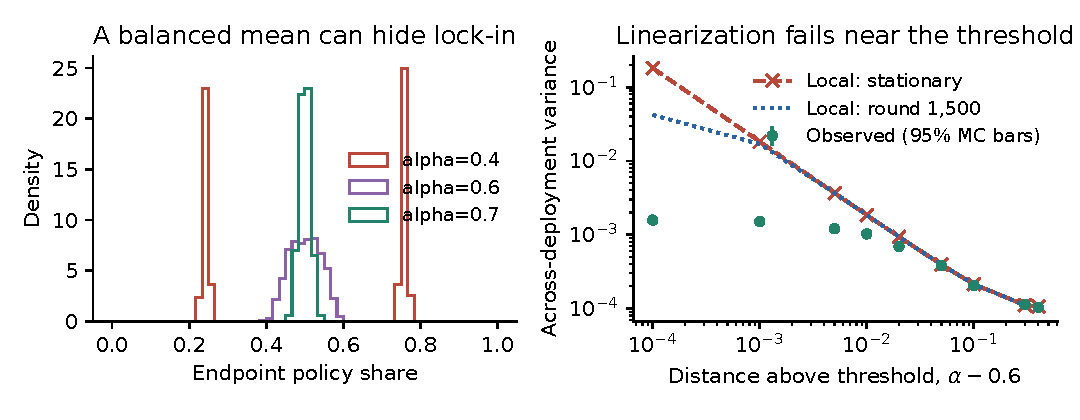
\includegraphics[width=\linewidth]{../results/participation_noise_camera_ready_v2.pdf}
\caption{Finite-feedback simulations, 2,000 deployments per condition after 1,500 rounds. Left: opposite lock-in directions can yield a mean near parity while each deployment is unrepresentative. Right: endpoint variance with approximate 95\% Monte Carlo bars ($\pm1.96$ MCSE), compared with local stationary and finite-horizon predictions. The logarithmic horizontal axis measures distance above $\alpha_c=.6$.}
\label{fig:noise}
\end{figure}

Figure~\ref{fig:noise} separates an ensemble statement from a deployment statement. Symmetry can keep average service near $1/2$ while each run settles far from parity. Mean absolute deviation detects this imbalance. The added scenarios also locate the approximation's boundary: at $\alpha=.6001$, observed variance is $.001573$ (MCSE $.000039$), versus stationary prediction $.182022$ and finite-horizon prediction $.042026$. At $.61$, observed variance $.001019$ is still 44.7\% below the local prediction; at $.65$, the discrepancy is only 3.1\%, comparable to its Monte Carlo uncertainty.

Longer runs do not close the near-threshold gap: at $.6001$, the 15,000-round variance is $.001629$ (MCSE $.000039$). The conditional mean has a restoring cubic term, $\mathbb{E}[e_{t+1}\mid e_t]=de_t-\lambda(1-\alpha)\beta^3e_t^3/6+O(e_t^5)$, and endogenous noise variance decreases away from parity. The linear prediction omits both effects. Deterministic stability therefore does not suffice for quantitatively accurate linear noise predictions. Appendix~\ref{app:simulation} reports all added scenarios and horizons; finite horizons alone do not establish stationarity.

\begin{table}[t]\centering
\caption{Finite-feedback endpoints at 1,500 rounds. Mean absolute deviation (MAD) measures within-deployment imbalance. Its MCSE is the sample standard deviation of absolute deviations divided by $\sqrt{2000}$. Uncertainty is conditional on the stated model. All quantities are policy shares.}
\label{tab:simulation}
\begin{tabular}{lrrr}\toprule
Audit weight $\alpha$ & Mean policy share & MAD & MCSE of MAD\\\midrule
0 & .49264 & .49290 & .00004\\
.4 & .50950 & .25758 & .00015\\
.6 & .50103 & .03380 & .00049\\
.7 & .49984 & .01142 & .00019\\
.9 & .49988 & .00843 & .00014\\
1 & .50005 & .00818 & .00013\\\bottomrule
\end{tabular}
\end{table}

Table~\ref{tab:simulation} makes the scale difference visible. At $\alpha=.4$, mean policy share is $.5095$ but mean absolute deviation is $.2576$: near-parity aggregation masks within-instance imbalance. At the critical weight $.6$, deterministic convergence coexists with a finite-feedback deviation of $.0338$; at $.7$, it falls to $.0114$. MCSEs quantify simulation precision, not uncertainty about human behavior.

Under the model's service interpretation, group utilities are $u_1(x)=x$ and $u_2(x)=1-x$. Mean utility is always $1/2$, while worst-group utility is $1/2-|x-1/2|$. Its mean is about $.2424$ at $\alpha=.4$ and $.4886$ at $.7$: average service can mask poor worst-group service. These model calculations motivate reporting within-instance representation alongside the aggregate mean.

Stability alone is not a welfare criterion. Performatively stable predictors can be suboptimal for the risk they induce~\citep{miller2021}, and static fairness constraints can have unfavorable downstream group effects~\citep{liu2018}. Our service utilities therefore make the evaluation target explicit rather than equating every stable fixed point with desirable alignment.

\paragraph{Allocating a fixed feedback budget.}
The two sample sizes and the effective audit weight are different design choices. Suppose a round can collect $B=n+m$ independent labels at equal per-label cost, while $\alpha$ is fixed by the desired stability margin. At parity, the innovation variance in Eq.~\eqref{eq:innovation} is minimized by
\begin{equation}
n=(1-\alpha)B,\qquad m=\alpha B,\qquad
\operatorname{Var}(\xi)=\frac{\lambda^2}{4B}.
\label{eq:allocation}
\end{equation}
For $0<\alpha<1$, this follows from
$((1-\alpha)^2/n+\alpha^2/m)(n+m)\geq((1-\alpha)+\alpha)^2=1$
by Cauchy--Schwarz, with equality when $n:m=(1-\alpha):\alpha$. Integer counts require feasible rounding; endpoint cases use only the nonzero-weight stream. This calculation assumes the local parity approximation and independent, equally costly labels.

With this allocation and $\gamma<1$, the local policy-variance approximation becomes
\begin{equation}
\operatorname{Var}(e)\approx\frac{\lambda}{4B(1-\gamma)[2-\lambda(1-\gamma)]}.
\label{eq:budgetvariance}
\end{equation}
Substituting $d=1-\lambda(1-\gamma)$ into Eq.~\eqref{eq:variance} gives the expression directly. It separates the amount of feedback, $B$, from the dynamic amplification factor. Doubling the label budget halves the predicted local variance, but it does not move the deterministic instability threshold. Increasing audit weight changes that threshold through $\gamma$, even if the total number of labels is unchanged. More endogenous feedback alone therefore cannot repair an unstable population-feedback loop in this model.

At fixed $\alpha$ in the strictly stable regime, smaller update rates reduce the predicted stationary variance but lengthen recovery. The deterministic relaxation time, measured in rounds for an $e$-fold decrease, is $-1/\log d$ for $0<d<1$. For $\beta=5$, $\alpha=.7$, and $\lambda=.35$, $d=.9125$ and this time is approximately 10.9 rounds. At the same audit weight with $\lambda=.1$, it is approximately 39.5 rounds. A system judged after only a few rounds can therefore look persistent even when its equilibrium is stable. Evaluation horizon, perturbation decay, and endpoint variability should be reported together.

Unequal collection costs change the allocation, not the algebraic feedback gain for a fixed effective weight. If endogenous and audit labels cost $k_e>0$ and $k_a>0$, respectively, a budget constraint is $k_e n+k_a m=C$. Minimizing the same local innovation variance gives $n/m=((1-\alpha)/\alpha)\sqrt{k_a/k_e}$, obtained by equating the two first-order conditions. The costlier stream receives fewer labels than under equal costs while retaining its declared weight, which increases sampling uncertainty. If recruitment also changes response behavior, the assumed participation function must be re-estimated; the formula does not cover that additional intervention.

Our simulations keep $n=m=500$ while varying $\alpha$, separating effective weight from sample count rather than implementing Eq.~\eqref{eq:allocation}. Table~\ref{tab:diagnosis} summarizes why this separation changes the appropriate intervention.

\begin{table}[t]\centering
\caption{Different mechanisms require different repairs. Predictions are not uniquely identifying tests; mechanisms can coexist. Bias and variance rows concern settled dynamics in the strictly stable, unique-attractor regime. More labels alone change neither feedback gain nor audit composition.}
\label{tab:diagnosis}
\begin{tabular}{p{.21\linewidth}p{.35\linewidth}p{.34\linewidth}}\toprule
Mechanism & Model prediction & Relevant intervention\\\midrule
Feedback instability & Near parity, perturbations amplify: $\gamma>1$. & Raise effective representative weight $\alpha$.\\
Audit-frame bias & At a biased attractor, displacement persists with more samples. & Correct audit composition $q$, not just its size.\\
Sampling noise & Fluctuations around the attracting target. & Increase label budget; smaller $\lambda$ trades recovery speed for precision.\\\bottomrule
\end{tabular}
\end{table}

\section{A measurement protocol for coupled alignment}\label{sec:measurement}
The estimand is the effect of own-group service on subsequent feedback provision, separately from any effect on preferences. A deployment study should start with a known invitation frame and an independently recruited measurement panel. Record invitation, exposure, response, voluntarily supplied group membership, pre-treatment preference, and measured feedback burden. Report the invited and responding populations separately. Data statements and datasheets offer useful structures for documenting population and collection choices~\citep{bender2018,gebru2021}; here their role is to make the dynamic sampling boundary auditable.

\paragraph{Identify participation before estimating feedback gain.}
Within a consented setting where the intervention is appropriate, randomize small changes to the deployed policy near the reference allocation, while keeping invitation probability independent of engagement. Estimate group-specific response probabilities conditional on the randomized exposure. The ratio in Eq.~\eqref{eq:ratio} implies a slope $2\beta$ for $\log r_1-\log r_2$ with respect to $x$; the derivative of respondent share at parity is instead $\beta/2$. Confusing these scales gives a factor-of-four error in the stability calculation. When groups have unequal population shares, use Eq.~\eqref{eq:unequalgain} rather than the symmetric formula.

Randomizing invitations alone identifies response rates under the existing policy but does not identify how policy changes them. Conversely, randomizing a displayed response only among currently active users need not identify the effect on people who have already disengaged. These are reasons to retain a population-based invitation frame and explicitly define the exposure population. Known invitation probabilities permit weighting only under overlap and suitable nonresponse assumptions; weighting cannot recover preferences from a group with no observable responses without additional information.

Performative power formalizes a system's causal ability to change participants' outcomes~\citep{hardt2022}. Randomized search-result arrangements provide a concrete example of measuring such effects on clicks~\citep{search2024}. Our target differs: estimate policy effects on feedback provision, then combine that response with the learner's sensitivity. A click effect, a response-rate effect, and the full feedback gain are not interchangeable estimands.

\paragraph{Calibrate the learner's part of the loop.}
The proportional update in Eq.~\eqref{eq:update} has target derivative one with respect to feedback composition. For a real large language model (LLM) alignment pipeline, let $h(p)$ be the deployed service allocation obtained from feedback share $p$ under the fixed training recipe. At a fixed point, write $p^*=(1-\alpha)p(x^*)+\alpha/2$ and $x^*=h(p^*)$. The local feedback factor becomes $(1-\alpha)h'(p^*)p'(x^*)$ when auditing mixes feedback before applying $h$. Thus a participation estimate alone is insufficient: controlled reweighting of an unchanged preference dataset can estimate $h'$ near the operating point. The policy metric, training randomness, and reference point must be declared in advance. If $h$ is not differentiable or scalar policy summaries are inadequate, the one-dimensional threshold is not an appropriate validation target.

For this generalized learner the full update is $x_{t+1}=(1-\lambda)x_t+\lambda h((1-\alpha)p(x_t)+\alpha/2)$. Writing $L=(1-\alpha)h'(p^*)p'(x^*)$, strict local stability requires $|1-\lambda+\lambda L|<1$; the simpler $L<1$ criterion presumes $L\ge0$. Representative parity also requires $h(1/2)=1/2$. Thus the operating point and the sign of the measured response must be checked before applying the symmetric threshold.

\paragraph{Test the intervention rather than infer it from attrition.}
A second randomization can assign independent system instances or sufficiently isolated cohorts to effective audit weights around the predicted threshold. The model predicts that the local persistence coefficient crosses \emph{one}, from amplification to contraction, as audit weight increases. It does not predict that the coefficient changes sign. Track perturbation decay, respondent composition, absolute policy deviation, and the least-observed group's coverage. Independent deployment units are needed because shared model updates create interference among users; treating thousands of labels from one model as independent system replications would exaggerate precision.

Before deployment, preregister the operating-point window, policy metric, grouping rule, response estimand, independent instances, and stopping rule. In this proposed study, a repeated panel would track within-person preference change while fresh samples track respondent composition. Comparing them requires measuring panel attrition; both channels may coexist.

\paragraph{Safeguards and actionable monitoring.}
Collect group information voluntarily, minimize its granularity, compensate recruited feedback, and report only adequately sized cells. Group labels should not be inferred from sensitive behavior solely to enforce a mathematical target. A stable but inaccurate audit frame can reproduce exclusion under the appearance of control. Monitoring should therefore include audit-frame drift and nonresponse, not only the estimated feedback coefficient. The observable warning signal is a growing discrepancy between invited population, responding population, and deployed service, interpreted alongside changes in preferences.

\section{Implications and limitations}
Representative recruitment and robust aggregation operate at different points in the pipeline. Group distributionally robust optimization (group DRO) protects against mixtures of represented groups~\citep{sagawa2020}, and robust preference objectives can protect heterogeneous feedback under their modeling assumptions~\citep{ramesh2024,chakraborty2024}. Clone-robust alignment addresses another sampling unit: near-duplicate alternatives rather than absent feedback providers~\citep{procaccia2025}. These are compatible with an independent recruitment stream. Protecting a group in an optimization objective does not by itself establish that its feedback remains observable, correctly labeled, or representative. Conversely, representative sampling does not resolve disagreement over how preferences should be aggregated.

The model fixes preferences, membership, and a shared service axis. Learning, strategic coordination, within-group disagreement, and history-dependent invitation costs require richer state variables. Positive participation response must be estimated: poor service can motivate complaints and a negative slope. Recruitment can also change response incentives rather than merely mix streams.

Human response functions and service targets require application-specific validation. Near the stability threshold, linear variance predictions also require an empirical accuracy check.

\section{Conclusion}
Alignment systems can alter not only the feedback they receive but the composition of those willing to provide it. In a participation-sensitive update loop, slowing learning and supplying representative evidence are different interventions. An effective audit weight can remove asymmetric attractors, while biased or finite audit feedback introduces distinct errors. Dynamic alignment should therefore evaluate the stability of its sampling process alongside the quality of its learned policy.

\clearpage
{\small
\begin{thebibliography}{99}
\bibitem[Bai et al.(2022)]{bai2022} Y. Bai et al. \href{https://arxiv.org/abs/2204.05862}{Training a Helpful and Harmless Assistant with Reinforcement Learning from Human Feedback}. arXiv:2204.05862, 2022.
\bibitem[Bender and Friedman(2018)]{bender2018} E. M. Bender, B. Friedman. \href{https://aclanthology.org/Q18-1041/}{Data Statements for Natural Language Processing: Toward Mitigating System Bias and Enabling Better Science}. \emph{Transactions of the Association for Computational Linguistics}, 6:587--604, 2018.
\bibitem[Brown et al.(2022)]{brown2022} G. Brown, S. Hod, I. Kalemaj. \href{https://proceedings.mlr.press/v151/brown22a.html}{Performative Prediction in a Stateful World}. \emph{AISTATS}, PMLR 151:6045--6061, 2022.
\bibitem[Chakraborty et al.(2024)]{chakraborty2024} S. Chakraborty, J. Qiu, H. Yuan, A. Koppel, D. Manocha, F. Huang, A. S. Bedi, M. Wang. \href{https://proceedings.mlr.press/v235/chakraborty24b.html}{MaxMin-RLHF: Alignment with Diverse Human Preferences}. \emph{ICML}, PMLR 235, 2024.
\bibitem[Chaney et al.(2018)]{chaney2018} A. J. B. Chaney, B. M. Stewart, B. E. Engelhardt. \href{https://doi.org/10.1145/3240323.3240370}{How Algorithmic Confounding in Recommendation Systems Increases Homogeneity and Decreases Utility}. \emph{ACM RecSys}, pp. 224--232, 2018.
\bibitem[Christiano et al.(2017)]{christiano2017} P. F. Christiano, J. Leike, T. Brown, M. Martic, S. Legg, D. Amodei. \href{https://proceedings.neurips.cc/paper_files/paper/2017/file/d5e2c0adad503c91f91df240d0cd4e49-Paper.pdf}{Deep Reinforcement Learning from Human Preferences}. \emph{NeurIPS}, 30, 2017.
\bibitem[Conitzer et al.(2024)]{conitzer2024} V. Conitzer et al. \href{https://arxiv.org/abs/2404.10271}{Social Choice Should Guide AI Alignment in Dealing with Diverse Human Feedback}. \emph{ICML}, PMLR 235, 2024.
\bibitem[De et al.(2026)]{de2026} S. De, I. Slaughter, J. Guo, Q.-Y. Cheng, J. Yan, S. Banerjee, M. Saveski. \href{https://arxiv.org/abs/2606.30905}{How Human Feedback Shapes AI-generated Community Notes}. arXiv:2606.30905, 2026.
\bibitem[Ensign et al.(2018)]{ensign2018} D. Ensign, S. A. Friedler, S. Neville, C. Scheidegger, S. Venkatasubramanian. \href{https://proceedings.mlr.press/v81/ensign18a.html}{Runaway Feedback Loops in Predictive Policing}. \emph{Conference on Fairness, Accountability and Transparency}, PMLR 81:160--171, 2018.
\bibitem[Falahati et al.(2026)]{falahati2026} A. Falahati, M. Mohammadi Amiri, K. Larson, L. Golab. \href{https://doi.org/10.1609/aaai.v40i44.41070}{The Alignment Game: A Theory of Long-Horizon Alignment Through Recursive Curation}. \emph{AAAI}, 40(44):37379--37386, 2026.
\bibitem[Fish et al.(2025)]{fish2025} S. Fish, P. G\"olz, D. C. Parkes, A. D. Procaccia, G. Rusak, I. Shapira, M. W\"uthrich. \href{https://arxiv.org/abs/2309.01291v3}{Generative Social Choice}. arXiv:2309.01291v3, 2025.
\bibitem[Ge et al.(2024)]{ge2024} L. Ge, D. Halpern, E. Micha, A. D. Procaccia, I. Shapira, Y. Vorobeychik, J. Wu. \href{https://proceedings.neurips.cc/paper_files/paper/2024/file/9328208f88ec69420031647e6ff97727-Paper-Conference.pdf}{Axioms for AI Alignment from Human Feedback}. \emph{NeurIPS}, 2024.
\bibitem[Gebru et al.(2021)]{gebru2021} T. Gebru, J. Morgenstern, B. Vecchione, J. Wortman Vaughan, H. Wallach, H. Daum\'e III, K. Crawford. \href{https://arxiv.org/abs/1803.09010v8}{Datasheets for Datasets}. \emph{Communications of the ACM}, 64(12):86--92, 2021.
\bibitem[Hardt and Mendler-D\"unner(2025)]{survey2025} M. Hardt, C. Mendler-D\"unner. \href{https://arxiv.org/abs/2310.16608v2}{Performative Prediction: Past and Future}. arXiv:2310.16608v2, 2025.
\bibitem[Hardt et al.(2022)]{hardt2022} M. Hardt, M. Jagadeesan, C. Mendler-D\"unner. \href{https://arxiv.org/abs/2203.17232v2}{Performative Power}. arXiv:2203.17232v2, 2022.
\bibitem[Hardt et al.(2023)]{hardt2023} M. Hardt, E. Mazumdar, C. Mendler-D\"unner, T. Zrnic. \href{https://proceedings.mlr.press/v202/hardt23a.html}{Algorithmic Collective Action in Machine Learning}. \emph{ICML}, PMLR 202, 2023.
\bibitem[Hashimoto et al.(2018)]{hashimoto2018} T. Hashimoto, M. Srivastava, H. Namkoong, P. Liang. \href{https://proceedings.mlr.press/v80/hashimoto18a.html}{Fairness Without Demographics in Repeated Loss Minimization}. \emph{ICML}, PMLR 80:1929--1938, 2018.
\bibitem[Jiang et al.(2019)]{jiang2019} R. Jiang, S. Chiappa, T. Lattimore, A. Gy\"orgy, P. Kohli. \href{https://doi.org/10.1145/3306618.3314288}{Degenerate Feedback Loops in Recommender Systems}. \emph{AIES}, pp. 383--390, 2019.
\bibitem[Kim et al.(2026)]{kim2026} K. Kim, J. Zhang, A. Ozdaglar, P. A. Parrilo. \href{https://arxiv.org/abs/2506.05619}{Beyond RLHF and NLHF: Population-Proportional Alignment Under an Axiomatic Framework}. \emph{ICLR}, 2026.
\bibitem[Kirk et al.(2024)]{kirk2024} H. R. Kirk et al. \href{https://arxiv.org/abs/2404.16019}{The PRISM Alignment Dataset: What Participatory, Representative and Individualised Human Feedback Reveals About the Subjective and Multicultural Alignment of Large Language Models}. \emph{NeurIPS Datasets and Benchmarks}, 2024.
\bibitem[Kleine Buening et al.(2025)]{kleine2025} T. Kleine Buening, J. Gan, D. Mandal, M. Kwiatkowska. \href{https://arxiv.org/abs/2503.09561}{Strategyproof Reinforcement Learning from Human Feedback}. \emph{NeurIPS}, 2025.
\bibitem[Liu et al.(2018)]{liu2018} L. T. Liu, S. Dean, E. Rolf, M. Simchowitz, M. Hardt. \href{https://proceedings.mlr.press/v80/liu18c.html}{Delayed Impact of Fair Machine Learning}. \emph{ICML}, PMLR 80, 2018.
\bibitem[Mendler-D\"unner et al.(2020)]{mendler2020} C. Mendler-D\"unner, J. C. Perdomo, T. Zrnic, M. Hardt. \href{https://proceedings.neurips.cc/paper/2020/file/33e75ff09dd601bbe69f351039152189-Paper.pdf}{Stochastic Optimization for Performative Prediction}. \emph{NeurIPS}, 33, 2020.
\bibitem[Mendler-D\"unner et al.(2024)]{search2024} C. Mendler-D\"unner, G. Carovano, M. Hardt. \href{https://arxiv.org/abs/2405.19073v2}{An engine not a camera: Measuring performative power of online search}. arXiv:2405.19073v2, 2024.
\bibitem[Miller et al.(2021)]{miller2021} J. Miller, J. C. Perdomo, T. Zrnic. \href{https://proceedings.mlr.press/v139/miller21a.html}{Outside the Echo Chamber: Optimizing the Performative Risk}. \emph{ICML}, PMLR 139, 2021.
\bibitem[Morris et al.(2019)]{morris2019} T. P. Morris, I. R. White, M. J. Crowther. \href{https://doi.org/10.1002/sim.8086}{Using simulation studies to evaluate statistical methods}. \emph{Statistics in Medicine}, 38(11):2074--2102, 2019.
\bibitem[Ouyang et al.(2022)]{ouyang2022} L. Ouyang et al. \href{https://arxiv.org/abs/2203.02155}{Training Language Models to Follow Instructions with Human Feedback}. \emph{NeurIPS}, 35:27730--27744, 2022.
\bibitem[Perdomo et al.(2020)]{perdomo2020} J. C. Perdomo, T. Zrnic, C. Mendler-D\"unner, M. Hardt. \href{https://proceedings.mlr.press/v119/perdomo20a.html}{Performative Prediction}. \emph{ICML}, PMLR 119:7599--7609, 2020.
\bibitem[Procaccia et al.(2025)]{procaccia2025} A. D. Procaccia, B. Schiffer, S. Zhang. \href{https://proceedings.mlr.press/v267/procaccia25a.html}{Clone-Robust AI Alignment}. \emph{ICML}, PMLR 267, 2025.
\bibitem[Rafailov et al.(2023)]{rafailov2023} R. Rafailov, A. Sharma, E. Mitchell, S. Ermon, C. D. Manning, C. Finn. \href{https://arxiv.org/abs/2305.18290}{Direct Preference Optimization: Your Language Model Is Secretly a Reward Model}. \emph{NeurIPS}, 36, 2023.
\bibitem[Ramesh et al.(2024)]{ramesh2024} S. S. Ramesh, Y. Hu, I. Chaimalas, V. Mehta, P. G. Sessa, H. Bou Ammar, I. Bogunovic. \href{https://proceedings.neurips.cc/paper_files/paper/2024/file/762b012aad39c011ff5606dcc8e140f8-Paper-Conference.pdf}{Group Robust Preference Optimization in Reward-free RLHF}. \emph{NeurIPS}, 2024.
\bibitem[Sagawa et al.(2020)]{sagawa2020} S. Sagawa, P. W. Koh, T. B. Hashimoto, P. Liang. \href{https://arxiv.org/abs/1911.08731}{Distributionally Robust Neural Networks for Group Shifts: On the Importance of Regularization for Worst-Case Generalization}. \emph{ICLR}, 2020.
\bibitem[Shumailov et al.(2024)]{shumailov2024} I. Shumailov, Z. Shumaylov, Y. Zhao, Y. Gal, N. Papernot, R. Anderson. \href{https://arxiv.org/abs/2305.17493v3}{The Curse of Recursion: Training on Generated Data Makes Models Forget}. arXiv:2305.17493v3, 2024.
\bibitem[Sun et al.(2025)]{sun2025} H. Sun, Y. Chen, S. Wang, X. Chu, W. Chen, X. Deng. \href{https://arxiv.org/abs/2405.16276}{Mechanism Design for LLM Fine-tuning with Multiple Reward Models}. \emph{NeurIPS}, 2025.
\bibitem[Suresh and Guttag(2021)]{suresh2021} H. Suresh, J. Guttag. \href{https://doi.org/10.1145/3465416.3483305}{A Framework for Understanding Sources of Harm throughout the Machine Learning Life Cycle}. \emph{ACM Conference on Equity and Access in Algorithms, Mechanisms, and Optimization}, 2021.
\bibitem[Xie and Zhang(2024)]{xie2024} T. Xie, X. Zhang. \href{https://proceedings.neurips.cc/paper_files/paper/2024/hash/e664650506f1cf2b4696df892147c06e-Abstract-Conference.html}{Automating Data Annotation under Strategic Human Agents: Risks and Potential Solutions}. \emph{NeurIPS}, 2024.
\end{thebibliography}}

\clearpage
\appendix
\section{Connecting invitation, response, and policy shares}\label{app:calibration}
The main model assumes equal invitation probabilities. To see why this matters, let group shares be $w$ and $1-w$, invitation probabilities be $\iota_1(x),\iota_2(x)>0$, and conditional response probabilities be $r_1(x),r_2(x)>0$. The respondent share and its log odds are
\begin{align*}
p_w(x)&=\frac{w\iota_1(x)r_1(x)}{w\iota_1(x)r_1(x)+(1-w)\iota_2(x)r_2(x)},\\
\log\frac{p_w(x)}{1-p_w(x)}&=\log\frac{w}{1-w}+\log\frac{\iota_1(x)}{\iota_2(x)}+\log\frac{r_1(x)}{r_2(x)}.
\end{align*}
Differentiation shows that a policy-dependent invitation ratio contributes to the respondent log-odds slope. Respondent composition alone cannot separate invitation and conditional-response contributions. Representative response at $x=w$ requires equal invitation--response products, not merely equal invitation counts. The main theorems continue to use their stated equal-invitation model.

For a concrete symmetric example, invite everyone ($\iota_1=\iota_2=1$) and take $\beta=5$, $x=.6$. Then $r_1=\sigma(1)=.7311$ and $r_2=.2689$, giving population-average response probability $.5$ but respondent share $.7311$. At $\lambda=.35$, the next service share is $.6459$ without audit and $.5893$ with $\alpha=.7$. Pooled response volume at the current state is unchanged, yet the audit reverses the policy's movement relative to parity. These are model calculations, not measured human responses.

\section{Criticality, unequal populations, and delayed feedback}\label{app:boundaries}
The critical symmetric expansion is $y_{t+1}=y_t-ky_t^3+O(y_t^5)$ with $k=\lambda\beta^2/12$. For a nonzero trajectory converging monotonically to zero,
\[
\frac{1}{y_{t+1}^2}-\frac{1}{y_t^2}
=\frac{(1-ky_t^2+O(y_t^4))^{-2}-1}{y_t^2}=2k+O(y_t^2).
\]
Averaging these increments gives $y_t^{-2}/t\to2k$, yielding the main paper's $t^{-1/2}$ rate. Exponential half-life formulas are therefore inappropriate at equality. A small residual after a finite simulation horizon is not evidence of a second deterministic attractor.

For the unequal-population example, roots of $x=(1-\alpha)\sigma(\log(w/(1-w))+2\beta(x-w))+\alpha w$ are bracketed on $[0,1]$ and refined by bisection. At $w=.2$, $\beta=5$, $\alpha=.5$, they are approximately $.20000$, $.28782$, and $.54230$. The first and third attract; the middle repels. The local feedback factor at $.2$ is $.8$, although a distant attractor remains. At $\alpha=.7$ the global feedback-target derivative bound $(1-\alpha)\beta/2=.75<1$ guarantees a contracting update and uniqueness, consistent with the root $.2$. At $\lambda=.35$, the full update derivative is bounded by $.9125$. The derivative bound, not numerical root search alone, supplies the global guarantee.

For one-round delay, linearized errors obey $e_{t+1}=(1-\lambda)e_t+\lambda\gamma e_{t-1}$. Its roots are
\[
z_\pm=\frac{1-\lambda\pm\sqrt{(1-\lambda)^2+4\lambda\gamma}}{2}.
\]
When $\gamma>0$, one root is positive and one negative. The positive root is below one exactly when $\gamma<1$; in that case the negative root is above $-1$, since the characteristic polynomial at $-1$ is $2-\lambda(1+\gamma)>0$. At $\gamma=0$, the roots are $0$ and $1-\lambda$. At equality $\gamma=1$, roots are $1$ and $-\lambda$: strict contraction fails, and the linearization alone cannot establish nonlinear critical stability. In particular, $\lambda=1$ also gives root $-1$. We do not extend the no-delay critical-rate result to this boundary.

\section{Simulation precision and the approximation near criticality}\label{app:simulation}
The simulation estimand is $\operatorname{Var}(x_T)$ across independent deployments under the declared update, not uncertainty in a fitted human-response parameter. Every condition starts at $x_0=.5$, uses $\beta=5$, $\lambda=.35$, $n=m=500$, and has $R=2{,}000$ deployments. Each round draws a fresh endogenous count from $\operatorname{Binomial}(500,p(x_t))$ and a fresh audit count from $\operatorname{Binomial}(500,.5)$. The two count vectors are independent, and draws use fresh randomness across rounds and deployments. Policy states within a deployment are temporally dependent. Endpoint variance uses denominator $R-1=1{,}999$.

\paragraph{Exact generator and draw order.}
The six original conditions use NumPy's \texttt{Generator(PCG64(20260904))} and run in the order $0,.4,.6,.7,.9,1$, without reseeding between conditions. Within a condition, rounds run in ascending order; at each round the generator draws the full endogenous vector in deployment-index order, then the full audit vector, and then updates all states simultaneously. Both vectors are drawn even if one stream has zero policy weight. Retaining these conventions reproduces Table~\ref{tab:simulation} and the original variance rows to printed precision.

The new conditions run in the order $.6001,.601,.605,.61,.62,.65$. They use separate \texttt{PCG64} streams from the six children of \texttt{SeedSequence(20261004).spawn(6)}, in that order. All use the same round-major draw convention. Each trajectory continues through rounds 1,500, 5,000, and 15,000; these checkpoints are paired within a deployment. Saved endpoint arrays and initial/checkpoint generator states permit direct inspection. The workflow uses Python 3.13.5, NumPy 2.3.5, and Matplotlib 3.10.8, with pinned dependencies.

\paragraph{Monte Carlo standard error of estimated variance.}
Let $s^2=(R-1)^{-1}\sum_j(x_{j,T}-\bar x_T)^2$. Write $s^2_{(-j)}$ for the sample variance after removing deployment $j$, using denominator $R-2$, and $\bar s^2_{(-)}=R^{-1}\sum_j s^2_{(-j)}$. We estimate
\begin{equation}
\widehat{\operatorname{MCSE}}(s^2)=
\left[\frac{R-1}{R}\sum_{j=1}^R
\left(s^2_{(-j)}-\bar s^2_{(-)}\right)^2\right]^{1/2}.
\label{eq:variance-mcse}
\end{equation}
This delete-one jackknife estimates uncertainty from finitely many independent deployments without assuming Gaussian endpoint shares. It is distinct from the deployment standard deviation $s$. Figure~\ref{fig:noise} uses approximate 95\% Monte Carlo bars $s^2\pm1.96\widehat{\operatorname{MCSE}}$; these quantify precision of a simulation summary, not a 95\% range for an individual deployment. Horizon contrasts use the same deletion index at both checkpoints, preserving their pairing. This follows the simulation-uncertainty distinction emphasized by \citet{morris2019}.

\begin{table}[htbp]\centering
\caption{Variance checks after 1,500 rounds, with all other original settings fixed. Variances and MCSEs are in units of $10^{-4}$. The local finite-horizon prediction is $V_\infty^{\rm lin}(1-d^{3000})$; the stationary column is Eq.~\eqref{eq:variance}. Relative discrepancy compares observed and stationary variance. The last three conditions reproduce the accepted results.}
\label{tab:variance-audit}
\newcommand{\variancerows}{%
0.6001 & 15.732 & 0.391 & 420.257 & 1820.220 & -99.1\%\\
0.601 & 14.990 & 0.376 & 169.036 & 182.220 & -91.8\%\\
0.605 & 12.001 & 0.311 & 36.624 & 36.624 & -67.2\%\\
0.61 & 10.194 & 0.276 & 18.428 & 18.428 & -44.7\%\\
0.62 & 6.869 & 0.197 & 9.336 & 9.336 & -26.4\%\\
0.65 & 3.781 & 0.115 & 3.900 & 3.900 & -3.1\%\\
0.7 & 2.031 & 0.064 & 2.123 & 2.123 & -4.3\%\\
0.9 & 1.122 & 0.036 & 1.101 & 1.101 & +1.9\%\\
1 & 1.033 & 0.031 & 1.061 & 1.061 & -2.6\%\\
}

\begin{tabular}{rrrrrr}\toprule
$\alpha$ & Observed & MCSE & Local, $T=1500$ & Local, stationary & Discrepancy\\\midrule
\variancerows
\bottomrule
\end{tabular}
\end{table}

Table~\ref{tab:variance-audit} directly tests conditions approaching $.6$ from above. At $.6001$, accounting for the finite horizon reduces the linear prediction from $.182022$ to $.042026$, but both remain far above the observed $.001573$. At $.605$ the finite-horizon and stationary predictions already agree to the displayed precision, yet the discrepancy remains 67.2\%. Thus insufficient settling of the linear recursion cannot explain the whole mismatch. At $.65$, the 3.1\% discrepancy is about one MCSE of the variance estimate; agreement is also close at $.7,.9,1$.

\begin{table}[htbp]\centering
\caption{Longer horizons for the six added conditions. Entries are observed variance $\pm$ one MCSE, in units of $10^{-4}$. Every column has 2,000 independent deployments; checkpoints share the same trajectories. These finite-horizon checks do not establish an exact stationary law.}
\label{tab:horizon}
\newcommand{\horizonrows}{%
0.6001 & 15.732 $\pm$ 0.391 & 15.928 $\pm$ 0.394 & 16.292 $\pm$ 0.395\\
0.601 & 14.990 $\pm$ 0.376 & 16.263 $\pm$ 0.401 & 16.334 $\pm$ 0.400\\
0.605 & 12.001 $\pm$ 0.311 & 13.162 $\pm$ 0.349 & 13.262 $\pm$ 0.345\\
0.61 & 10.194 $\pm$ 0.276 & 9.614 $\pm$ 0.270 & 9.922 $\pm$ 0.280\\
0.62 & 6.869 $\pm$ 0.197 & 7.588 $\pm$ 0.226 & 7.079 $\pm$ 0.202\\
0.65 & 3.781 $\pm$ 0.115 & 3.660 $\pm$ 0.108 & 3.801 $\pm$ 0.123\\
}

\begin{tabular}{rrrr}\toprule
$\alpha$ & $T=1500$ & $T=5000$ & $T=15000$\\\midrule
\horizonrows
\bottomrule
\end{tabular}
\end{table}

For $.601$ and $.605$, the increase from 1,500 to 15,000 rounds is about 2.5 and 2.8 paired MCSEs, respectively, so some finite-horizon variation is detectable. Nevertheless, at 15,000 rounds their observed variances remain $.001633$ and $.001326$, far below stationary predictions $.018222$ and $.003662$. The near-threshold approximation gap therefore persists after a tenfold increase in horizon.

The nonlinear conditional mean restores more strongly away from parity through the negative cubic term stated in Section~\ref{sec:noise}. Moreover, its endogenous innovation variance contains $p(x_t)(1-p(x_t))/n$, which is at most $1/(4n)$ and decreases away from parity. The local model replaces it by its value at parity. Both approximations matter when fluctuations leave the linear neighborhood. At $\alpha=1$ the mean update is linear and the stationary variance expression is exact; remaining discrepancies arise from Monte Carlo uncertainty. At or below the threshold, the linear stationary prediction is not evaluated.

The complete workflow, including exact replay of the original results, checks, figures, and added scenarios, took 26.4 seconds on an Apple Silicon central processing unit (CPU). It uses no trained model, external dataset, or service. The accompanying code contains a single entry point, the full draw conventions, saved arrays, environment information, and executable checks; a fresh output directory prevents accidental overwriting.

\section{Separating a stability budget from a sampling budget}\label{app:budget}
Write $a=1-\alpha$. With label costs $k_e,k_a>0$ and total expenditure $C=k_en+k_am$, Cauchy--Schwarz gives
\[
\left(\frac{a^2}{n}+\frac{\alpha^2}{m}\right)(k_en+k_am)
\ge(a\sqrt{k_e}+\alpha\sqrt{k_a})^2.
\]
For $0<\alpha<1$, equality yields $n/m=(a/\alpha)\sqrt{k_a/k_e}$. At endpoint weights, allocate to the sole nonzero-weight stream. The minimum local innovation variance is $\lambda^2(a\sqrt{k_e}+\alpha\sqrt{k_a})^2/(4C)$. Effective weight is fixed and reweighting is allowed; this neither chooses the welfare target nor repairs audit bias. Integer counts require feasible rounding.

At equal costs, $B=1000$ and $\alpha=.7$, the allocation is $(n,m)=(300,700)$ rather than the simulated $(500,500)$. The parity innovation coefficient $a^2/n+\alpha^2/m$ falls from $.00116$ to $.00100$, a 13.79\% reduction. The feedback gain remains $.75$ in either design. This is a conditional variance calculation, not an additional simulation result. The saved experiments intentionally hold both sample sizes fixed while varying effective audit weight, isolating a different design question.


\end{document}
